% A simple template for Beamer presentations in LaTeX
% 
% To produce pdf run:
%   $ pdflatex beamer.tex 

\documentclass{beamer}
\usetheme{Singapore}

% Bibliography
%\usepackage{cite}
\usepackage{biblatex}


\hypersetup{colorlinks=true}

% Show table of contents between sections
\AtBeginSection[]
{
  \begin{frame}
    \frametitle{Table of Contents}
    \tableofcontents[currentsection]
  \end{frame}
}

% Graphics examples
%\centerline{\includegraphics[height=2.5in]{figs/normal.pdf}}
%\includegraphics[width=4in]{figs/makefile.png}

%%%%%%%%%%%%%%%%%%%%%%%%%%%%%%%%%%%%%%%%%%%%%%%%%%%%%%%%%%%%

\begin{document}

\title{Parallel Computing Through Code Analysis}
\date{\today}
\date{10 May 2017}
\author{Clark Fitzgerald}
\institute{UC Davis - Statistics Student Seminar}
\titlegraphic{\includegraphics[height=.5\textheight]{../workflow.pdf}}

\frame{\titlepage}

\begin{frame}
    \frametitle{Outline}
    \tableofcontents
\end{frame}

%%%%%%%%%%%%%%%%%%%%%%%%%%%%%%%%%%%%%%%%%%%%%%%%%%%%%%%%%%%%
\section{Motivating Example}
%%%%%%%%%%%%%%%%%%%%%%%%%%%%%%%%%%%%%%%%%%%%%%%%%%%%%%%%%%%%
\begin{frame}

    \frametitle{Loop detectors count cars, measuring velocity and
    occupancy}

\centerline{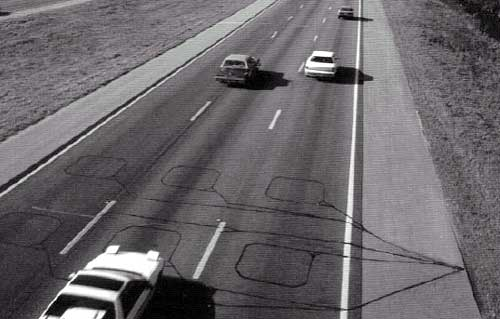
\includegraphics[height=2.5in]{loop_detector.jpg}}

\end{frame}
%%%%%%%%%%%%%%%%%%%%%%%%%%%%%%%%%%%%%%%%%%%%%%%%%%%%%%%%%%%%
\begin{frame}

\frametitle{Caltrans Performance Measurement System (PeMS) records this
data for the whole state}

    \begin{itemize}
        \item Each sensor measures 3 quantities
        \item Data point every 30 seconds
        \item $43,680$ sensors in California
        \item $\implies$  377 million data points per day
    \end{itemize}

\end{frame}
%%%%%%%%%%%%%%%%%%%%%%%%%%%%%%%%%%%%%%%%%%%%%%%%%%%%%%%%%%%%
\begin{frame}

    \frametitle{Traffic engineers study the relationships between variables
    \cite{li2011fundamental}}

\centerline{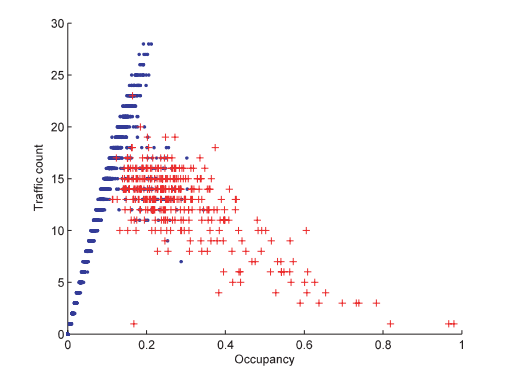
\includegraphics[height=2.5in]{fundamental_diagram.png}}

\end{frame}
%%%%%%%%%%%%%%%%%%%%%%%%%%%%%%%%%%%%%%%%%%%%%%%%%%%%%%%%%%%%
\begin{frame}

    \frametitle{Using more data allows new types of analyses}

    \begin{itemize}
        \item Effect of policy such as speed limits and carpool lanes
        \item Impact of road features such as on/off ramps
        \item Effect of weather
        \item Clustering detectors
    \end{itemize}

    % Policy is especially interesting, because that can potentially be changed
    % Recommending state wide policy, then why not look at data for the
    % whole state?

\end{frame}
%%%%%%%%%%%%%%%%%%%%%%%%%%%%%%%%%%%%%%%%%%%%%%%%%%%%%%%%%%%%
\begin{frame}[fragile]

    \frametitle{R expresses statistical computation well}

\centerline{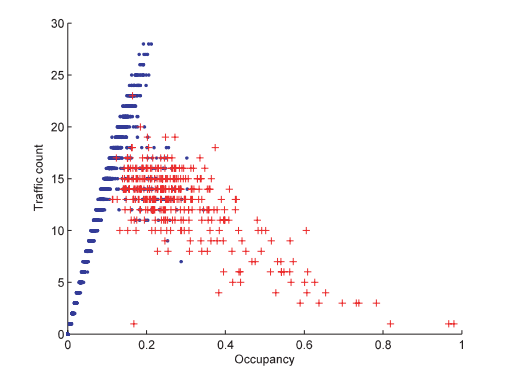
\includegraphics[height=2in]{fundamental_diagram.png}}

\begin{verbatim}
by(data, INDICES = station, FUN = piecewise_rlm)
\end{verbatim}

% This is a good reason to stay with R, for that matter.

\end{frame}
%%%%%%%%%%%%%%%%%%%%%%%%%%%%%%%%%%%%%%%%%%%%%%%%%%%%%%%%%%%%
\begin{frame}

    \frametitle{Parallel code allows computation on larger data sets}

    \pause
    But it can distract from the research question.

%\end{frame}
%%%%%%%%%%%%%%%%%%%%%%%%%%%%%%%%%%%%%%%%%%%%%%%%%%%%%%%%%%%%%
%\begin{frame}
%
%    \frametitle{Lets scale up the computations with parallel programming}
%
%    \begin{itemize}
%        \item Several parallel strategies exist to improve performance
%        \item Which is best depends on the platform and data
%        \item Each one requires deeper knowledge of that particular technology
%        \item Therefore techniques to programmatically identify and use the parallel
%  patterns implicit in code would be valuable
%    \end{itemize}

\end{frame}
%%%%%%%%%%%%%%%%%%%%%%%%%%%%%%%%%%%%%%%%%%%%%%%%%%%%%%%%%%%%
\section{Simple Example}
%%%%%%%%%%%%%%%%%%%%%%%%%%%%%%%%%%%%%%%%%%%%%%%%%%%%%%%%%%%%
\begin{frame}[fragile]

\frametitle{Illustrate different parallel computational models}

Consider computing the mean,

\begin{equation}
    \bar{x} = \frac{1}{n} \sum_{i = 1}^n x_i
\label{eq:mean}
\end{equation}

where the $x_i$'s are i.i.d. $\sim N(0, 1)$. 
    
In R this code is written:

\begin{verbatim}
xbar = mean(rnorm(n))
\end{verbatim}

\end{frame}
%%%%%%%%%%%%%%%%%%%%%%%%%%%%%%%%%%%%%%%%%%%%%%%%%%%%%%%%%%%%
\begin{frame}

    \frametitle{This can also be expressed as a weighted mean}

\begin{equation}
    \bar{x} = \frac{1}{n} \sum_{j = 1}^p \sum_{i = 1}^{n_j} x_{ij}
    = \sum_{j = 1}^p \frac{n_j}{n} \bar{x}_j
\label{eq:mean_partial}
\end{equation}

Suppose that all $n_j$'s are the same for the following examples.

\end{frame}
%%%%%%%%%%%%%%%%%%%%%%%%%%%%%%%%%%%%%%%%%%%%%%%%%%%%%%%%%%%%
\begin{frame}[fragile]

    \frametitle{The weighted mean can be directly translated into R code}

\begin{verbatim}
meanrnorm = function(n) mean(rnorm(n))

partial_means = sapply(rep(n_i, p), meanrnorm)
xbar = mean(partial_means)
\end{verbatim}

\pause 

    \begin{itemize}
        \item While not parallel, this effectively removes the memory limits.
        \item How to choose the $n_i$ and $p$?
    \end{itemize}

\end{frame}
%%%%%%%%%%%%%%%%%%%%%%%%%%%%%%%%%%%%%%%%%%%%%%%%%%%%%%%%%%%%
\begin{frame}[fragile]

    \frametitle{The same computation can be evaluated on many workers
    simultaneously}

\centerline{\includegraphics[height=2in]{../snow.pdf}}

\begin{verbatim}
parallel::clusterCall(cluster, meanrnorm, n_i)
\end{verbatim}

\end{frame}
%%%%%%%%%%%%%%%%%%%%%%%%%%%%%%%%%%%%%%%%%%%%%%%%%%%%%%%%%%%%
\begin{frame}[fragile]

    \frametitle{Pipeline parallelism is like a factory assembly line.}

\centerline{\includegraphics[width=\textwidth]{../pipeline.pdf}}

\begin{verbatim}
# Worker 1
x_chunk = rnorm(n_i)
serialize(x_chunk, worker2)


# Worker 2
x_chunk = unserialize(worker1)
partial_means[i] = mean(x_chunk)
\end{verbatim}

\end{frame}
%%%%%%%%%%%%%%%%%%%%%%%%%%%%%%%%%%%%%%%%%%%%%%%%%%%%%%%%%%%%
\section{Code Analysis}
%%%%%%%%%%%%%%%%%%%%%%%%%%%%%%%%%%%%%%%%%%%%%%%%%%%%%%%%%%%%
\begin{frame}[fragile]

    \frametitle{Idiomatic R already expresses computation in a natural
    parallel way through ``apply'' functions.}

\begin{verbatim}
x = replicate(5, rnorm(n_i), simplify = FALSE)

partialmeans = lapply(x, mean)

by(data, INDICES = station, FUN = piecewise_rlm)
\end{verbatim}

%    Specifically: apply, lapply, sapply, tapply, by, mapply, Map, vapply,
%    replicate, outer

\end{frame}
%%%%%%%%%%%%%%%%%%%%%%%%%%%%%%%%%%%%%%%%%%%%%%%%%%%%%%%%%%%%
\begin{frame}

    \frametitle{Layers mark ways for users to write parallel code for one
    platform}

\begin{itemize}
    \item \textbf{User Layer}: foreach, future, partools, ddR, biganalytics, RevoScaleR
    \item \textbf{R layer}: SNOW, parallel, bigmemory, Rmpi
    \item \textbf{System Layer}: processes, *NIX fork(), memory maps, network sockets,
    MPI
\end{itemize}

\end{frame}
%%%%%%%%%%%%%%%%%%%%%%%%%%%%%%%%%%%%%%%%%%%%%%%%%%%%%%%%%%%%
\begin{frame}

    \frametitle{How can we transform R code into a lower layer?}

\begin{itemize}
    \item \textbf{Plain old R code: \texttt{lapply(), sapply(), for(), \dots}}
\item User Layer: foreach, future, partools, ddR, biganalytics, RevoScaleR
\item R layer: SNOW, multicore, parallel, bigmemory, Rmpi
\item System Layer: processes, *NIX fork(), memory maps, network sockets,
    MPI
\end{itemize}

% Potentially we can transform to any of these layers

%\end{frame}
%%%%%%%%%%%%%%%%%%%%%%%%%%%%%%%%%%%%%%%%%%%%%%%%%%%%%%%%%%%%%
%\begin{frame}
%
%   \frametitle{Preserving language semantics can be challenging.}
%
%    For example, R's dynamic lookups 
%
%\begin{verbatim}
%
%    f = function() 0
%    g = function() f() + 1
%    f = function() 10
%    g()                     # Returns 11!
%
%\end{verbatim}

\end{frame}
%%%%%%%%%%%%%%%%%%%%%%%%%%%%%%%%%%%%%%%%%%%%%%%%%%%%%%%%%%%%
\begin{frame}

    \frametitle{(Code, Data, Platform) together determine the execution
    strategy}

    \begin{itemize}
    \item \textbf{Code} script to be executed
    \item \textbf{Data} in-memory, files, database, etc
    \item \textbf{Platform} 4 core laptop, server with GPU, Spark cluster
    \end{itemize}

\end{frame}
%%%%%%%%%%%%%%%%%%%%%%%%%%%%%%%%%%%%%%%%%%%%%%%%%%%%%%%%%%%%
\begin{frame}[fragile]

    \frametitle{One challenge is how to properly abstract ``data''}

    Some options:

    \begin{itemize}
        \item Iterators of chunks as in R's \texttt{iterators} package
        \item ``file-like'' objects from *NIX
        \item Pick one serialization format, ie. CSV, feather
        \item Abstract parallel data structures
    \end{itemize}

    \pause

    \begin{itemize}
        \item Maintain custom metadata objects?
        \item Only focus on data frames / tables?
    \end{itemize}

\end{frame}
%%%%%%%%%%%%%%%%%%%%%%%%%%%%%%%%%%%%%%%%%%%%%%%%%%%%%%%%%%%%
\begin{frame}

    \frametitle{An iterator produces data on demand}

    \centerline{\includegraphics[height=2in]{../iterator.pdf}}

    \begin{itemize}
        \item Most flexible of the above options
        \item Natural in pipeline parallel model
        \item Operate well with high performance IO libraries
    \end{itemize}



    % Iterators are appealing for pipelined parallelism, and for using an
    % underl

%\end{frame}
%%%%%%%%%%%%%%%%%%%%%%%%%%%%%%%%%%%%%%%%%%%%%%%%%%%%%%%%%%%%%
%\begin{frame}
%
%    \frametitle{Map and reduce functions}
%
%    Let $f: x \rightarrow y$ and $x = O(n)$, a data structure with $O(n)$
%    elements.
%
%    \begin{itemize}
%        \item If $y$ is also $O(n)$ then we can call $f$ a \textbf{Map} function.
%
%        \item Example: $f(x) = 2x$ for $x \in R^n$.
%
%    % This is vectorization in R
%    
%        \item If $y$ is $O(1)$ then $f$ is a \textbf{Reduce} function.
%
%        \item Example: $f(x) = \sum_{i = 1}^n x_i$
%    \end{itemize}

\end{frame}
%%%%%%%%%%%%%%%%%%%%%%%%%%%%%%%%%%%%%%%%%%%%%%%%%%%%%%%%%%%%
\begin{frame}

\frametitle{Parallel processing comes with overhead}

    \centerline{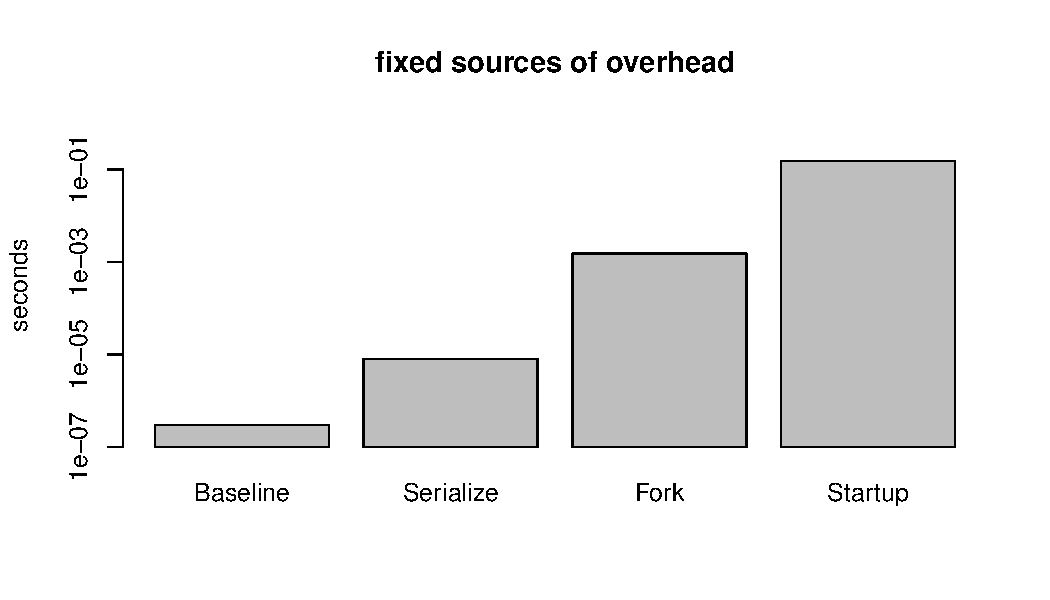
\includegraphics[height=2.5in]{../compute_times/overhead}}

% If there wasn't any overhead, we would use it all the time for
    % everything.

% So if you start up a process, you want to keep it around

\end{frame}
%%%%%%%%%%%%%%%%%%%%%%%%%%%%%%%%%%%%%%%%%%%%%%%%%%%%%%%%%%%%
\begin{frame}


    \frametitle{Creating efficient code as a constrained optimization
    problem}

\textbf{Parameters}
\begin{itemize}
    \item number of processor cores to use
    \item size of each chunk
    \item which functions to combine in one processing step
\end{itemize}

\textbf{Constraints}
\begin{itemize}
    \item number of cores available
    \item network bandwidth
    \item disk IO speed
    \item available memory
\end{itemize}

\end{frame}
%%%%%%%%%%%%%%%%%%%%%%%%%%%%%%%%%%%%%%%%%%%%%%%%%%%%%%%%%%%%
\begin{frame}

    \frametitle{One version of the optimization problem}

    % TODO: Get Duncan's feedback
\begin{itemize}
    \item $w_i$ worker startup time
    \item $c(x_i)$ communication time to send $x_i$ and receive $f(x_i)$.
    \item $e(x_i)$ time to evaluate $f(x_i)$ on a worker.
\end{itemize}

Then we minimize
\[
    \max_{x_i} w_i + c(x_i) + e(x_i)
\]
for $x = (x_1, \dots, x_m)$, a partition of $x$ into chunks.

\end{frame}
%%%%%%%%%%%%%%%%%%%%%%%%%%%%%%%%%%%%%%%%%%%%%%%%%%%%%%%%%%%%
\begin{frame}

    \frametitle{If we want to compute on out of memory data:}

\begin{itemize}
    \item $w$ worker startup time
    \item $l$ latency in communication
    \item $t(n_i)$ time to compute on $n_i$ elements
    \item $m(n_i)$ memory required to compute on $n_i$ elements
\end{itemize}

Then we minimize
\[
    w + 2l + \max (t(n_i))
\]
such that 

\begin{itemize}
    \item $\sum n_i = n$ total data points
\end{itemize}


\end{frame}
%%%%%%%%%%%%%%%%%%%%%%%%%%%%%%%%%%%%%%%%%%%%%%%%%%%%%%%%%%%%
\begin{frame}

    \frametitle{Compiled R code provides even more efficiency}

    This work will complement efforts to compile R.

Probably follow the OpenCL kernel model.

\end{frame}
%%%%%%%%%%%%%%%%%%%%%%%%%%%%%%%%%%%%%%%%%%%%%%%%%%%%%%%%%%%%
\section{Conclusion}
%%%%%%%%%%%%%%%%%%%%%%%%%%%%%%%%%%%%%%%%%%%%%%%%%%%%%%%%%%%%

\begin{frame}

    \frametitle{Follow up on the sensor example}

    Program should:

\begin{enumerate}
    \item Remove any observations it can
    \item Reorganize files on disk based on station ID
    \item Apply function to each station ID file
\end{enumerate}

\end{frame}
%%%%%%%%%%%%%%%%%%%%%%%%%%%%%%%%%%%%%%%%%%%%%%%%%%%%%%%%%%%%
\begin{frame}

    \frametitle{Some support infrastructure is necessary}

\begin{itemize}
\item Use profiling and microbenchmark to measure overhead
\item A file sort from R
\end{itemize}


\end{frame}
%%%%%%%%%%%%%%%%%%%%%%%%%%%%%%%%%%%%%%%%%%%%%%%%%%%%%%%%%%%%
\begin{frame}

    \frametitle{Next Steps}

    The larger data sets are very interesting. 

    Solving the right problem...
    
    How can we come back
    to statistics? Norm keeps pushing me back to thinking about the 

\end{frame}
%%%%%%%%%%%%%%%%%%%%%%%%%%%%%%%%%%%%%%%%%%%%%%%%%%%%%%%%%%%%
\begin{frame}

    \frametitle{More Applications}

\begin{itemize}
    \item Benford test on election campaign contribution data
        \cite{tam2007breaking}
    \item Forest greenness satellite imagery (Andrew Latimer)
    \item Simulating spread of disease (Nistara Randhawa)
\end{itemize}

\end{frame}
%%%%%%%%%%%%%%%%%%%%%%%%%%%%%%%%%%%%%%%%%%%%%%%%%%%%%%%%%%%%
\begin{frame}

    \frametitle{Acknowledgements}

\begin{itemize}
    \item Feedback from Duncan Temple Lang and Nick Ulle
    \item Applications from Data Science Institute Affiliates
\end{itemize}

\end{frame}
%%%%%%%%%%%%%%%%%%%%%%%%%%%%%%%%%%%%%%%%%%%%%%%%%%%%%%%%%%%%
\begin{frame}

    \frametitle{Questions?}
    \centerline{\includegraphics[height=2.5in]{../workflow.pdf}}

\end{frame}
%%%%%%%%%%%%%%%%%%%%%%%%%%%%%%%%%%%%%%%%%%%%%%%%%%%%%%%%%%%%
\begin{frame}

    \frametitle{Additional Slides}

\end{frame}
%%%%%%%%%%%%%%%%%%%%%%%%%%%%%%%%%%%%%%%%%%%%%%%%%%%%%%%%%%%%
\begin{frame}

    \frametitle{The weighted mean can be directly translated into R code}

%%%%%%%%%%%%%%%%%%%%%%%%%%%%%%%%%%%%%%%%%%%%%%%%%%%%%%%%%%%%
%%%%%%%%%%%%%%%%%%%%%%%%%%%%%%%%%%%%%%%%%%%%%%%%%%%%%%%%%%%%
%%%%%%%%%%%%%%%%%%%%%%%%%%%%%%%%%%%%%%%%%%%%%%%%%%%%%%%%%%%%

\end{frame}
\begin{frame}
\frametitle{References}
\printbibliography
\end{frame}

\end{document}
